\documentclass[11pt]{article}
\usepackage{a4, fullpage}
\usepackage{bibtopic}
%\usepackage[small,compact]{titlesec}
\usepackage{float}
\usepackage{amssymb,amsmath}
\usepackage[T1]{fontenc}
\usepackage{graphicx}
\usepackage{multicol}
\restylefloat{table}
%\usepackage{parskip}
%\usepackage{setspace}

%\setlength{\parskip}{0.3cm}
%\setlength{\parindent}{0cm}
%\setlength{\textheight}{10in}
%\setlength{\textwidth}{6.5in}
%\setlength{\parskip}{2pt}
%\addtolength{\oddsidemargin}{-.3in}
%\addtolength{\evensidemargin}{-.3in}
%\addtolength{\topmargin}{-.6in}
%\addtolength{\textwidth}{.6in}

%Crowdsourcing of tasks has become very popular. It is often based on the principle that by having many different contributors to performing a task, an accurate and appropriate result will be achieved. The classical example is wikipedia where popular pages tend to be more accurate than less popular one. But contributions to a task do not always come for free and frameworks such as Amazon's mechanical turk allow for monetary rewards to be paid in exchange for contributing or performing a task. It is therefore the case that fewer contributions from more trustworthy contributors is more effective than many contributions from less trustworthy sources. 

%The aim of the project is to design and implement a framework that allows the optimum number of contributors to be selected on the basis of their trustworthiness for a desired accuracy of the outcome/result and that evaluates the trustworthiness of contributors on the basis of the accuracy of the results they provide.


\begin{document}



\title{Crowdtrust - Trustworthy Information From The Crowd\\ Group Project }

\author{Giovanni Charles \and Adam Fiksen \and Ryan Jackson \and Sahil Jain \and John Walker \and \\ Emil Lupu}

\date{\today}         % inserts today's date

\maketitle           % generates the title from the data above
\newpage

\begin{abstract}
\noindent Outsourcing is becomming increasingly popular in a lot of areas and as a result providing these required services has 
become big business. Companies are using the Internet to accept jobs from requestors which often require some human intelligence 
such as tagging images, they then distribute these jobs to a crowd of workers and return the results to the requestor. This process is called
crowdsourcing. %Not happy with this
\\
\\
\noindent At the moment Amazons \emph{Mechanical Turk} is the only real crowdsourcing `giant' in the market, with over 500,000 workers it offers
anyone with a computer and internet connection the ability to `earn \$\$\$ while working from home!'. Requestors (companies or individuals) 
can then submit a HIT(Human Intelligence Task) to the mechanical turk system, this HIT is then displayed to all users along with a 
reward for its completion, the results are then sent back to the requestor and they decide whether the work is worth paying for. 
This system raises a problem though, How do I know how accurate my results are? You have no control over which worker selects your HIT and
your task of 'Transcribe this podcast' could be carried out by a lacklustre employee in India who doesn't speak very good English. The solution
most requestor guides offer is to submit your job to multiple workers but this pushes up your costs linearly and leaves you to make a difficult
decision to make on the number of workers to consult.
\\
\\
We seek to create is a solution to this problem by providing a framework in which requesters can submit jobs with a required level of accurary. Our
system then decides how many users it needs to consult to achieve this based on their expertise. 
  
\end{abstract}

\newpage

\tableofcontents	%Do contents page and a 1 page break afterward

\newpage

%%%%%%%%%%%%%%%%%%%%%%%%%%%%%%%%%%%%%%%%%%%%%%%%%%%%%%%%%%%%%%%%%%%%%%%%%%%%%%%%

\section{Executive Summary}

\subsection{What is our product?}
Let's say that I have a 100 photos of birds, and I want to know which birds are 
robins, but I have no prior knowledge of birds. Our product, CrowdTrust, focusses
on fixing this problem.

Our product provides a framework where a person can submit a task and specify
the level of accuracy they want achieved in the task. After some calculations,
the total number of users which need to be sent the task is calculated, and
then the task is sent out to the optimum number of people. At the moment,
there is only one main competitor in the market, which is Amazon's Mechanical
Turk. What differentiates our product from Mechanical Turk is the fact that
we send out the task to an optimum number of people, which means the user
would eventually part away with less money for an accuract result.

So how does our product tie in with the problem previously proposed?I can go on 
CrowdTrust, upload the photos of birds and ask the question "Which of these are 
robins?". I would then specify the level of accuracy I want to achieve, and then 
the task is sent out to the crowd. Once completed, I get the solution to the 
task as proposed by the crowd as to which birds are robins.

\subsection{Why now?}
Crowdsourcing is become more popular day by day. It allows a person who needs
a job done, but has no prior knowledge on the subject, to get a very accurate
result through the contribution of many people who might be experts on the
subject of the task. Besides Mechanical Turk, there are other websites which
provide a specialised crowdsourcing frameworks, such at Stack Overflow. We wanted
to produce a framework which would not necessarily be specialised. The scope of
problems people face with today is large, and we wanted to take advantage of this.

\subsection{Why would you want it?}
There are two types of users who can use CrowdTrust. Firstly, there is the client,
who is the person who submits a task which needs answering. A client would want
to join because they could receive an accurate solution to a problem which they
wanted solving. Also, in the future, when paying the crowd is implemented,
using CrowdTrust could be significantly cheaper than Mechanical Turk. The second
type of user are the crowd members. Crowd members would want to join because
they might have a passion for solving problems. With the scope of CrowdTrust,
the types of problems you solve is massive. As mentioned, eventually, the crowd
would also be paid for solving tasks, which would be a primary reason as to why
someone would solve problems.
%%%%%%%%%%%%%%%%%%%%%%%%%%%%%%%%%%%%%%%%%%%%%%%%%%%%%%%%%%%%%%%%%%%%%%%%%%%%%%%%
\newpage
\section{Introduction}
%Set the scene ( motivation )
%State the problem you are trying to solve ( Ojective(s) )
%Summarise what you achieved ( contributions )
%%%%%%%%%%%
\subsection{What Is Crowdsourcing} %Change the I adam and 'I' will kill you
Our project concerns \emph{crowdsourcing} 'the book' would describe crowdsourcing as the principle of obtaining an accurate 
and appropriate result by having many different contributors performing a task but we'd like to start with a story which
we believe encapsulates the idea of crowdsourcing in its most positive and useful light.
\\
\\
In January 2009 Timothy Gowers (Fields Medal winner and avid blogger) used his blog to post a striking question \emph{Is massively 
collaborative mathematics possible?}. He posted a difficult and unsolved mathematical problem he was particularly interested in and invited 
people to contribute to its solution in the comments section. The project initally got off to a slow start but once the ice was broken the 
comments flooded in. 37 days , 27 contibuters and 800 comments later Timothy Gowers was able to announce that not only had they solved the 
original problem but they had also solved a harder generalisation of it, he called his experiment the \emph{Polymath Project} .
\\
\\
This is a nice example of how crowd sourcing can be used to combine the skills of many individuals and produce answers to a complex problems,
but there are many motivations to outsource your task to the crowd:
\begin{itemize}
\item
\emph{Computational Difficulty:} Timothy Gowers provided a nice example of a computationally difficult problem It is extememly unlikely you
would be able to write a Java program or use Wolphram Alpha to produce a complex mathematical proof, some problems require what we like to call
the 'human touch'. Problems which require the human touch are in no way confined to the realms of complex mathematics identifing an unknown
bird in a picture for example would prove quite difficult on a computer you may need access some a program like Google Goggles but even then you 
would probablly need a good quality photograph, whereas one avid bird enthusiast in the crowd might be able to easilly identify the bird and
reuturn the correct answer.
\item
\emph{Saving Time:} In 2009 aviator Steve Fosset crash landed deep in the Nevada desert, his friends knew they had a very small
and time critical window to find him alive and they had little faith in the current search and resuce operations. They organised for satellite 
images to be taken of the desert and the images were passed to a crowd who were asked to identify foreign object which could be potential crash 
sites. This is a nice example of how the crowd can be used to literally cover a large ammount of ground in a small ammount of time. Not all 
examples of saving time are quite this dramatic though, image tagging is an extemely arduous task for an individual or small group of people 
to perform and tagging a relatively large set of images could take weeks or even months, outsourcing this to the crowd could have the job 
done in a number of hours.
\item
\emph{Saving Money:} Time is money as they say and this goes hand it hand with the point above. If you have to pay a team of high salary computing
professionals to tag images for your project when you could be paying them to write code this is not cost effective, however passing this job off
to a crowd of lower paid people could potentially save you a lot of money. 
\item
\emph{Reaching A Willing Audiance:} Unless it's something they enjoy the fact is that people are not willing to work for free, this is why
getting the general public to do things such as complete surverys can be difficult as a large number of people will simply not want to do it. The
crowd memebers will be inventivised to perform work and as such will be more likely to complete your survey.
\end{itemize}
%%%%%%%%%%%
\subsection{Analysis of the Marketplace}

%%%%%%%%%%%
\subsection{Problem Description}
\begin{enumerate}
\item
\emph{How do we get these problems to the crowd?} 
\\
It is unlikely many people with a problem to be solved would want to go to the trouble
of creating a crowd themselves as this would be comparitive to the complexity of the problem itself therefore there is a need for a third party
crowd management system. 
\item
\emph{What problems can we ask the crowd?} 
\\
Specialised crowds have been successful and certainly have their uses for instance\\
www.stackoverflow.com can be thought of as a crowd specialising in the solution of computing problems, however it is unlikely I would
be able to find a specialised crowd to indentify bird pictures or to search satellite images for crash sites, therefore I need access 
to a generalised crowd able to adapt to and solve a wide variety of problems. The crowd management party therefore needs to provide
the ability to ask a wide variety of questions and the ability to easily encorporate new questions in response to new technology. %EMBELISH?
\item
\emph{How many people do we ask, who do we ask and how can we trust what they say?} 
\\
Crowd members will be a representitive sample of the general 
population, some will be brighter than others and some will be willing to put in more effort than others based on this you can place all 
annotators on a scale of trustworthiness which rates how much you believe an answer they give you. This rasises the question of 'how many 
people do I ask?', is consulting a small number of very trustworthy people better than a large number of non trustworthy people?, However I 
can't simply ask the same subset of people over and over again as workload will build up and my answers will be delayed. If I have a 
'specialist' question do I direct it to someone with knowledge of that specialism? Clearly a sophisticated algorithm is needed on the crowd
management side to address these problems. 
\end{enumerate}
A solution to these problems provides us with the basis for our project we are to:
\\
\\
\emph{Design and implement a framework that allows the optimum number of contributors to be selected on the basis of their trustworthiness 
for a desired accuracy of the outcome/result and that evaluates the trustworthiness of contributors on the basis of the accuracy of the 
results they provide.}
%%%%%%%%%%%
\subsection{Formal Objectives}
%%%%%%%%%%%
\subsection{Achievements}


%%%%%%%%%%%%%%%%%%%%%%%%%%%%%%%%%%%%%%%%%%%%%%%%%%%%%%%%%%%%%%%%%%%%%%%%%%%%%%%%
%\newpage
\section{Design and Implementation}
% Detail your design why did you do it this way?
%Summarise Key implementation details (how did you do it what 
%tools did you use

\subsection{Data Processing}

Once clients have submitted their tasks and the crowd are submitting answers, our goals are:
\begin{enumerate}
\item To estimate the correct annotation for each subtask based on crowd annotations and their respective likelihoods of being correct.
\item To use crowd annotations to better our understanding of the accuracy of a crowd
\end{enumerate}

These goals can be achieved with the `Expectation-Maximisation algorithm'. We have adopted this algorithm for the processing of annotations, generalised it to work over a variety of task types and implemented it to function efficiently in an online environment.\\

\subsubsection{EM-Algorithm overview}

The a EM algorithm models the system as a hypothesis, h, and new evidence, Y, which is a set independent instances with observed data, X, and unobserved data, Z.

For our particular case we have a set of subtasks, S, with correct annotations, $Z_{s}$; a set of annotators, J, with accuracies $A_{j}$ and labels $L_{ij}$ from these annotators to subtasks

It then iterates through two steps to revise this hypothesis so that it converges on the most likely hypothesis for the state of the system.\\

Expectation Step:\\
You calculate P(Z) values using the X assuming the current hypothesis holds. In our case Z are the correct annotations for each subtask, X are the provided labels and the current hypothesis is the annotator`s accuracy. [1]\\

$ p(z_{i}) = p(z_{i}|\zeta) \prod p (l_{ij} | z_{i} a_{j}) $ (1)\\

where $p(z|\zeta)$ is our prior belief of $p(z)$.\\

Maximisation Step:\\
You replace the current hypothesis h with the most likely hypothesis assuming that the Z = E[Z]. This will mean that we have to calculate our most likely accuracies for the system based on the expected correct annotations calculated from the previous step.\\

$ Q(a_{j},a\prime_{j}) = \log p(a_{j}|\alpha_{j}) + \sum E_{z_{i}} [\log p (l_{ij} | z_{i} a_{j})]$ (2)\\

\subsubsection{Annotation types}

Our framework deals with a variety of subtasks that have different annotation types and models for accurate behaviour.

We model each of the subtasks with a different conjugate prior and model for accurate behaviour.\\

%\renewcommand{\arraystretch}{1.5}
\begin{table}[htdp]
\caption{Subtask models [2]}
\begin{center}
\begin{tabular}{|p{2cm}|p{5cm}|p{4cm}|p{4cm}|}
Subtask type & Description & conjugate prior & likelihood \\
\hline
Binary & An annotator can respond either true or false & $Beta(\alpha_{j}^{0}, \beta_{j}^{0})Beta(\alpha_{j}^{1},\beta_{j}^{1})$, where $\alpha_{j}^{0/1}$ are the negative and positive successes and $\beta_{j}^{0/1}$ are the failures.& $p(l_{ij} = z_{i} = 1 | a_{j}) = a_{j}^{1}$ $p(l_{ij} = z_{i} = 0 | a_{j}) = a_{j}^{0}$\\ [2cm]

Multivalued & An annotator must categorise the subject into one of a range of categories D & $Beta(\alpha, \beta)$, where $\alpha$ is the number of successes and $\beta$ the failures.  &  $p(l_{ij} = z_{i}| a_{j}) = a_{j}$ $p(l_{ij} \ne z_{i} | a_{j}) = \frac{1 - a_{j}}{D - 1}$\\ [1cm]

Continuous & An annotator must respond using a tuple from an N-dimensional number line & as above &  $p(l_{ij} | z_{i} a_{j}) = a_{j} p(l_{ij}|honest) + (1- a_{j}) p(l_{ij}|random)$, where the probability of an honest label is given by $\mathcal{N}(l_{ij}, \sum)$ for a given variance and the random probability is uniform over the response space.\\
\end{tabular}
\end{center}
\label{models}
\end{table}

\subsubsection{Online Considerations}

The online implementation of this algorithm is different in that it does not compute the expected labels as a batch job but instead has to observe several instances, one at a time, over a long period of time.

It also exploits discrimination. Expert annotators are asked first to respond to subtasks in order to reduce the total number of labels required. Since experts are likely to be the minority this technique is important since it makes sure that their annotations are taken into account [3].

We carry this out by checking the variance of our estimate for the most likely accuracy of an annotator. A large variance would suggest that we do not yet have enough information to judge an annotator. When the variance is small enough, we will test the accuracy against the criteria below.\\

\begin{table}[htdp]
\caption{default}
\begin{center}
\begin{tabular}{|c|c|}
Subtask type & criteria\\ \hline
Binary & \shortstack{$\frac{\Phi^{-1}(a_{j}^{0}) - \Phi^{-1}(1 - a_{j}^{1})}{2} > 2$ \\ i.e an annotator's sensitivity index [1] is greater than 2}\\
Multivalued & $a_{j} > 0.85$\\ 
Continuous & $a_{j} > 0.85$\\
\end{tabular}
\end{center}
\label{default}
\end{table}%

\subsubsection{Implementation details}

\begin{figure}[htbp]
\begin{center}
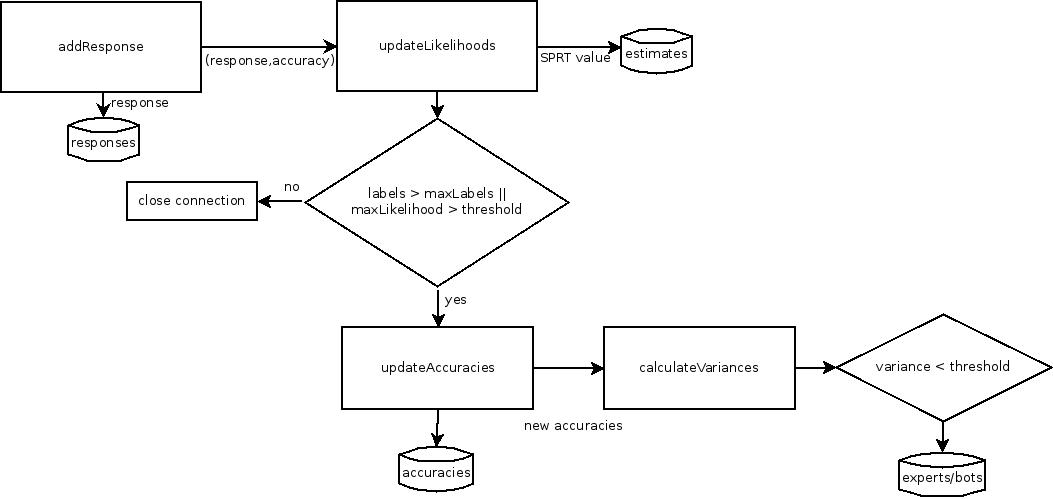
\includegraphics[width=\linewidth]{flow.jpg}
\caption{algorithm}
\label{default}
\end{center}
\end{figure}


E step\\

To calculate (1), values for the Sequential Probability Ratio Test [4] for each hidden value Z are stored in the database. Since the value is the sum of a sequence, the stored value can simply be increased by the new value. At this point each value is tested with the threshold to see if the maximum likelihood is great enough. At this point the M step will begin.\\

M step\\

To compute the new accuracy (2), the prior accuracy needs to be modelled as a distribution stated in figure 1 and the expected accuracy is calculated assuming the correct label is the most likely one from the last step.

The new accuracy would be the peak of the equation (2). To avoid using numerical methods to estimate the peak we write the Bayes estimate as a convex combination of the prior and the data [5]. This way we get a formula for the expected accuracy that can be computed in constant time:\\

\begin{table}[htdp]
\caption{Bayes estimate}
\begin{center}
\begin{tabular}{|c|c|c|}
Subtask type & Convex combination & $\theta_{mle}$\\ \hline

Binary & $ E(a_{j}^{k}) = \gamma \frac{\alpha_{j}^{k}}{\alpha_{j}^{k} + \beta_{j}^{k}} +  (1 - \gamma)\theta_{mle}$, only for affected k & 1 if $l_{ij} = z_{i}$, 0 otherwise\\

Multivalued & $ E(a_{j}) = \gamma \frac{\alpha_{j}}{\alpha_{j} + \beta_{j}} +  (1 - \gamma)\theta_{mle}$ &1 if $l_{ij} = z_{i}$, 0 otherwise\\

Continuous & $ E(a_{j}) = \gamma \frac{\alpha_{j}}{\alpha_{j} + \beta_{j}} +  (1 - \gamma)\theta_{mle}$ & \shortstack{$\frac{\mathcal{N}(l_{ij}| z_{i}, \sum)}{\mathcal{N}(l_{ij}| z_{i}, \sum) + \lambda^{-1}}$ \\ where $\lambda$ is the response space}\\
\end{tabular}
\end{center}
\label{def}
\end{table}%

where $\gamma = \frac{\alpha_{j}^{k} + \beta_{j}^{k}}{\alpha_{j}^{k} + \beta_{j}^{k} + 1}$ 

Once the accuracies have been updated we must check the variance of the posterior accuracy. In the cases where the accuracy is modelled as a single beta distribution, multi valued and continuous, is trivial:

In the binary case the accuracy is modelled as a product of two dependant distributions therefore the variance must be estimated. We fit the peak to a multivariate Gaussian curve to estimate the posterior`s variance.

If we are confident in our knowledge of the annotator we test its accuracy against the criteria and store any new data about experts and bots in the database.\\

%[1]  Machine Learning Tom M Mitchell
%[2] - A Compendium of Conjugate Priors - John D. Cook
%[3]  Online crowdsourcing: rating annotators and obtaining cost-effective labels - Welinder Perona
%[4] - Sequential tests of statistical hypotheses  Wald
%[5]  Bayesian inference for simple problems - Simon Jackman

 
%%%%%%%%%%%%%%%%%%%%%%%%%%%%%%%%%%%%%%%%%%%%%%%%%%%%%%%%%%%%%%%%%%%%%%%%%%%%%%%% 
%\newpage
\section{Evaluation}
%summarise testing procedures (+ relevant testing results)
\subsection{Testing}
\subsubsection{Validity}
Validity testing ensures our system can handle erroneous events, below are the validity tests we carried out:
\begin{itemize}
\item
\item
\end{itemize}
\subsubsection{Security}
Security testing ensures our system conforms to the appropriate security standards, below are the security tests we carried out:
\begin{itemize}
\item
\item
\end{itemize}
\subsubsection{Scaleability}
Scalability testing ensures the system can handle increased demand, below and the scalability tests we carried out:
\begin{itemize}
\item
\item
\end{itemize}
\subsubsection{Performance}
Performance testing ensures the system performs in a timely manner, below are the performance tests we carried out: 
\begin{itemize}
\item
\item
\end{itemize}
\subsubsection{Correctness}
Correctness testing ensures the system outputs what it is supposed to, below are the correctness tests we carried out:
\begin{itemize}
\item
\item
\end{itemize}
\subsubsection{End To End}
End to end testing ensures a process makes its journey correctly through the system, below are the end to end tests we carried out:
\begin{itemize}
\item
\item
\end{itemize}

%Evaluate your deliverables in terms of performance usability
%usefulness, (how successful was the project?)

%%%%%%%%%%%%%%%%%%%%%%%%%%%%%%%%%%%%%%%%%%%%%%%%%%%%%%%%%%%%%%%%%%%%%%%%%%%%%%%%
%\newpage
\section{Conclusion and Future Extensions}
%Say what you've concluded from doing the work and how you'd build on it

%%%%%%%%%%%
\subsection{Conclusion}

%%%%%%%%%%%
\subsection{Future Extensions}

%%%%%%%%%%%%%%
\subsubsection{Tagging}
Tagging could be used to improve the efficency of our algorithm, for instance when a user signs up to the website he could provide a list of his
interests such as football or birdwatching and when a client submitts a task to the website he uses a similar tagging system to record what his
task is related to. If a user provides an answer to a task which is in line with his interests then it is more likely his answer will be correct
the algorithm would take this into account when calculating how sure it is of an answer. This will result in less people having to be asked 
for each question which will improve turnaround time for jobs submitted to the system. 


%%%%%%%%%%%%%%
\subsubsection{Dynamic Pricing Model}
If you do any reading into Amazons Mechanical Turk it's not long before you will meet some criticisms on the way they pay their workers with some
even likening it to an electronic sweat shop. The average wage for a worker is around \$2 far below the minimum wage and the average payment for 
a task is around 30 cents, whats more the requestor is under no obligation to pay the worker unless he is completely satisfied this is often abused
with companies simply choosing not to pay the workers. Workers really have no control over their wage and the ammount they are paid simply 
reflects how quickly they can complete tasks, crowdtrust could be used to change this.

With crowdtrust you keep track of an annotators 'expertise' and so you can return an answer to a task with a mesaure of how sure you are of its
correctness, this means users will not have to submit tasks multiple times to validate them this saves the user money and as a result some of this
saving could be passed on to the annotators to reward them for being experts.   

%%%%%%%%%%%%%%
\subsubsection{Mobile Access}
Althought Mechanical Turk has over 500000 workers registerd 80\% of HITs are performed by around 20\% of the workforce and this isn't a 
particularly large number. The reason for this we believe is the pay, if you're at home there are many things you'd rather be doing than sitting
if front of your computer for \$2 an hour. However if you're stuck on a 4 hour train journey from Newcastle back to London for university and
you could have access to a crowdtrust app on your phone you may be far more willing to sit there and earn \$8. We believe a mobile app would 
greatly increase the userbase and therefore the turn around time for tasks submitted to the system. 

%%%%%%%%%%%%%%%%%%%%%%%%%%%%%%%%%%%%%%%%%%%%%%%%%%%%%%%%%%%%%%%%%%%%%%%%%%%%%%%%
%\newpage
\section{Project Management}
%Planning, group organisation, breakdown + task allocation etc

%%%%%%%%%%%%%%%%%%%%%%%%%%%%%%%%%%%%%%%%%%%%%%%%%%%%%%%%%%%%%%%%%%%%%%%%%%%%%%%%
%\newpage
\section{Appendix}
%e.g user guide

%%%%%%%%%%%%%%%%%%%%%%%%%%%%%%%%%%%%%%%%%%%%%%%%%%%%%%%%%%%%%%%%%%%%%%%%%%%%%%%%
%\newpage
\begin{thebibliography}{9}

\end{thebibliography}

\end{document}

